\documentclass[conference]{IEEEtran}
% *** GRAPHICS RELATED PACKAGES ***
%
\ifCLASSINFOpdf
  % \usepackage[pdftex]{graphicx}
  % declare the path(s) where your graphic files are
  % and their extensions so you won't have to specify these with
  % every instance of \includegraphics
  % \DeclareGraphicsExtensions{.pdf,.jpeg,.png}
\else
  % or other class option (dvipsone, dvipdf, if not using dvips). graphicx
  % will default to the driver specified in the system graphics.cfg if no
  % driver is specified.
  % \usepackage[dvips]{graphicx}
  % declare the path(s) where your graphic files are
  % \graphicspath{{../eps/}}
  % and their extensions so you won't have to specify these with
  % every instance of \includegraphics
  % \DeclareGraphicsExtensions{.eps}
\fi

\usepackage{cite}
\usepackage{times}
\usepackage{wrapfig}
\usepackage{tweaklist}
\usepackage{xspace}
\usepackage{graphicx}
\usepackage{tabularx}
\usepackage{amsmath}
\usepackage{amssymb}
\usepackage{url}
\usepackage{bm}
\usepackage{color}
\usepackage{colortbl}
\usepackage{subfig}
\usepackage[ruled,vlined]{algorithm2e}

% correct bad hyphenation here
\hyphenation{op-tical net-works semi-conduc-tor}
\graphicspath{{../master_thesis/}}

\newcommand{\todo}[1]{\textbf{\textcolor{red}{TODO: #1}}}
\begin{document}
%
% paper title
% can use linebreaks \\ within to get better formatting as desired
\title{Contracting Curve Density Algorithm for Applications in Personal Robotics}


% author names and affiliations
% use a multiple column layout for up to three different
% affiliations
\author{\IEEEauthorblockN{Shulei Zhu and Dejan Pangercic and Michael Beetz}
\IEEEauthorblockA{Intelligent Autonomous Systems Group, TU Munich \\
Email: \{shulei.zhu, pangercic, beetz\}@cs.tum.edu}
}

% make the title area
\maketitle

\begin{abstract}
This paper investigates an extended and optimized
implementation of the state-of-the-art local curve fitting algorithm
named Contracting Curve Density (CCD) algorithm, originally developed 
by Hanek et al. In particular, we investigate its application  
in the field of personal robotics for the tasks such as the segmentation
of objects in clutter and the tracking of objects. 
The developed system mainly consists of two functional parts, the CCD
algorithm to fit the model curve in still images and the CCD tracker to
track the model in the videos. We demonstrate algorithm's working 
in various scenes using handheld camera and the cameras from the 
PR2 robot. Achieved results show that the CCD algorithm achieves 
robustness and sub-pixel accuracy even in the presence of clutter, 
partial occlusion, and changes of illumination.
\end{abstract}

\IEEEpeerreviewmaketitle

\section{Introduction}
The CCD algorithm can be best described as follows. Given one or multiple images as input
data and a parametric curve model with a priori distribution of model
parameters, through curve-fitting process, we estimate the model
parameters which determine the approximation of the posterior
distribution in order to make the curve models best matching the image data.

The curve-fitting problem and its variants have a wide range of
applications in the field of robotics, medical processing, user
interface, surveillance and biometrics~\cite{hanek2004fitting}. In order to be
widely applicable to practical personal robotics problems (such as
perception of mobile manipulation), robustness,
accuracy, efficiency and versatility should be
considered when a novel approach is designed and implemented.
However, in the computer vision community, solving object segmentation and the
related object contour tracking problems are always challenging,
especially in natural and unconstrained scenes. Due to clutter,
shading, texture, and highlights it is very difficult to segment
an object from an inhomogeneous background. Furthermore, some physical
conditions, such as the illumination or surface properties, will
influence the efficiency and stability of related approaches. It is
necessary and significant to develop a method which determines adequate segmentation
in advance or a single criterion that is applicable for all parts of objects boundaries.

\begin{figure}[htbp]
  \centering
  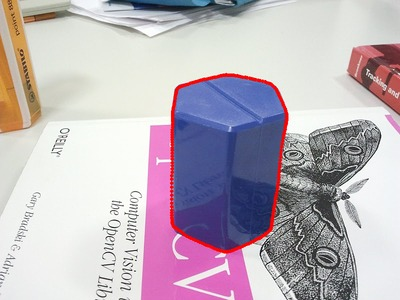
\includegraphics[width=\columnwidth]{images/divide1.jpg}\\
  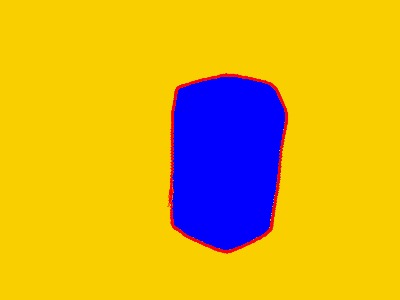
\includegraphics[width=\columnwidth]{images/divide2.jpg}
  \caption[A classification problem]{A classification problem: Top) The red
    contour successfully segment the box from the background. Bottom) The
    blue one is outside, the golden one is inside.}
  \label{fig:divide}
\end{figure}

\subsection{An Alternative View of the CCD Algorithm}
\label{sec:overview}

In the field of pattern recognition, the key concept is that of
uncertainty. In image data, the uncertainty arises both
through noise from measurements, as well as through the nature of
the objects (e.g. cardiac motion and deformation). Probability theory
provides a consistent framework for the quantification and
manipulation of uncertainty.  In this section, we view curve-fitting
problem from a probabilistic perspective and turn us towards to
a classification problem.

In the CCD algorithm, we aim to find the contour of observed object
and thus segment it from the background. Therefore, a hypothetical 
contour divides the image into two part (Fig.\ref{fig:divide}), inside
and outside. For probabilistic model, we can represent this using
binary representation (e.g. $\{0, 1\}$). The goal of the CCD algorithm
is to accurately
assign a class label to each pixel in the image (Actually, we only need assign those pixels in the vicinity of the
contour), thus the curve-fitting problem becomes a classification
one. A powerful approach to solve this problem involves modeling a
conditional probability distribution in an inference stage, and then
subsequently uses this distribution to make optimal decisions. In
order to derive the conditional probability, prior distribution and
likelihood function should be given.

We assume that a parametric curve model is governed by a prior distribution
over the model parameters (usually a multi-dimensional vector). There
exists a range of probability distributions which can be used to model
the distribution of shapes. In this paper, for simplicity, let us
consider the Gaussian distribution, which is commonly used in computer
vison because of its several outstanding features. 

Defining the prior distribution is only a step of the problem.
According to the Bayesian theorem, the conditional distribution
is proportional to the product of prior distribution and the likelihood
function. Hence, the next step is to define the likelihood function.

In the implementation of the CCD algorithm, it is suggested to use
local image pixels as the training data to determine the
likelihood function. If the data is assumed to be drawn  independently
from the distribution, then the likelihood function is given by the accumulation of all the components.
By pixel value we denote the vector containing the local single-or multichannel
image data associated to a pixel. In our experiments, we directly use the sensed RGB
values as pixel values. However, other types of local features computed in a pre-processing
step may also be used, e.g. texture descriptors or color values in
other color spaces.

The likelihood function obtained from the local statistics has
not a closed-form solution. In addition, the prior distribution is just
an approximate to the true distribution. Therefore, Maximization
likelihood method does not work here, we have to use an alternative
approach known as iterative reweighted least squares (IRLS) to find
the solution. Here the IRLS process is called Maximum a Posterior (MAP).

In the CCD algorithm, because we just need a parameter vector determining
the shape of specified contour, we do not plan to calculate the
predictive distribution. Therefore, the MAP solution mentioned above
is our objective.

However, take account into the fact that exact inference for the
regression is always intractable, we have encountered some issues before
implementing the algorithm. In the next section, we will discuss these
problems.

\subsection{Contributions}
In order to improve the stability, accuracy and robustness over the original
implementation we introduce the following novel improvements. Firstly, we use the logistic sigmoid
function instead of a Gaussian error function which renders a
curve-fitting problem as a Gaussian logistic regression problem known in the
field of pattern recognition. Secondly, a quadratic or
a cubic B-spline curve is used to model the parametric curve
to avoid the Runge phenomenon without increasing the degree of the
B-spline. Thirdly, the system supports both planar affine (6-DOF) and
three-dimensional affine (8-DOF) shape-space. The latter affine space can avoid
curve mismatching caused by major viewpoint changes. Lastly, in
order to avoid manual intervention by the user, the developed system
also supports robust global initial curve initialization modules based on both keypoint
feature matching and back-projections from the 3D point clouds.

\todo{In the remainder of this document ...}
\section{Related Work}
\todo{Shorten significantlly}\\
We split this section based on the following criteria:
\begin{itemize}
\item Articles on two-dimensional and three-dimensional deformable models,
  such as Snakes and gradient vector flow deformable models;
\item Articles on applying statistical knowledge to the models.
\end{itemize}

\subsection{Two-dimensional \& Three-dimensional Models}
\label{sec:23m}
Many traditional segmentation methods are effected by the assumption that the
images studied in computer vision are usually self-contained, namely,
the information needed for a successful segmentation can be extracted
from the images.

In 1980s, a paradigm named \textit{Active Vision}~\cite{aloimonos1988active} escaped this bind and
pushed the vision process in a more goal-directed fashion. After that, a
notably successful departure, the \textit{Snakes}, is proposed in a
seminar work conducted by Kass~\cite{kass1988snakes}. The original paper, spawned many variations
and extensions including the use of Fourier
parameterisation~\cite{scott1987alternative}, and incorporation
of a topologically adaptable models~\cite{mcinerney1995topologically},
thereof application~\cite{mcinemey1999topology} and incorporation of a discrete
dynamic contour model~\cite{lobregt1995discrete}. A realization of the
Snakes using B-splines was developed in~\cite{brigger2000b}. In two
dimensions, the Snakes have a variation named active shape
model~\cite{cootes1995active}, which is a discrete version of this
approach. Gradient Vector Flow~\cite{xu1998snakes}, or GVF, is an extension developed
based on a new type of external field. In~\cite{xu2000gradient}
authors are concerned with the convergence properties of deformable
models. In three dimensions, a good deal of research work has been
conducted on matching three-dimensional models, both on rigid
~\cite{harris1993tracking} and deformable~\cite{terzopoulos1991dynamic} shapes.
\subsection{Applications}
\label{sec:app}
Model-based segmentation methods are widely used in the field of
medical image processing. Besides the segmentation,
dynamic models, such as the Snakes and its variations, are greatly used in application of object
tracking. A real-time tracking system based on deformable models, such
as the Snakes, is developed
in~\cite{terzopoulos1992tracking}. It proved that the active shape and
motion estimators are able to deal very effectively with the complex
motions of nonrigid objects. Furthermore, the combination of active
models and Kalman filter theory is also a popular approach to
tracking, some work about this can be found
in~\cite{schick1991simultaneous}. And last but not least,
~\cite{blake1998active} is a complete volume about the topics of
geometric and probabilistic models  for shapes and their dynamics.

\section{Statistical Models}
\label{sec:sm}
Pattern recognition theory is a general statistical framework which is
important in the study of model-based approaches. This has started from the 1970s
and 1980s when a new interpretation of image was proposed in the
statistical community.  Analyzing the model problems in probabilistic
context has two great advantages. The first is that it approaches the
nature of the problems, the ranges of shapes are defined by a
probability, this provides another viewpoint for the curve-fitting problem
in the field of computer vision. Another advantage is that when we
solve the problem in the field of pattern recognition, there are abundant tools to deal with such problems. 
The CCD approach is a method developed in the probabilistic context. 

In~\cite{kelemen1999three} and~\cite{kelemen1999elastic}, an elegant
use of statistical models for the segmentation of medical images is
designed.  The resulting segmentation system consists of building
statistical models and automatic segmentation of new image data
sets by restricting elastic deformation of models.  The works
in~\cite{sclaroff2001deformable} and~\cite{liu1999deformable} also
exploit the prior knowledge from the perspective of probability,
furthermore, the statistical shape models enforce the prior
probabilities on objects by designing a complicated energy function.  
In this paper, we assume that the shapes' priors have a Gaussian form in
shape-space. In the case of a norm-squared density over  quadratic spline space,
the prior is a Gaussian Markov Random Field
(MRF)~\cite{blake1998active}, which is used widely  for modeling
prior distributions for curves~\cite{storvik1994bayesian}.

Defining a prior distribution for shape is only part of the
problem, prior knowledge only controls the feature interpretation in an
image, also it just approximates the contour of an observed object. In
order to solve the problem, likelihood function is required. In some
special cases, we can get a solution by maximizing likelihood, but
usually it is intractable because there is no closed-solution. An indirect
approach known as iterative reweighted least squares
(IRLS)~\cite{bishop2006pattern} is used find the parameters of the model.
the CCD  algorithm uses local statistics to evaluate a conditional distribution
, then the iterative maximum a posteriori probability (MAP)
~\cite{sorenson1980parameter} estimate process is used to refine
parameters instead of maximizing a complicated cost function. 
Moreover, a blurred curve model is proposed as a efficient mean for iteratively optimizing. The algorithm
can be used in object localization and object tracking. As an example
of applications of the CCD approach, an efficient, robust and fully
automatic real-time system for 3D object pose tracking in
image sequences is presented in~\cite{panin2006fully}
and~\cite{panin2006efficient}. MultiOcular Contracting Curve Density
algorithm (MOCCD)~\cite{hahn2007tracking} is an extension of the CCD
approach. In the paper, it is integrated into the tracking system of
the human body. 

Both the Snakes and CCD can be used to build naive tracking
system. However, they are limited by the performance and stability
problems. Several methods achieve a speed-up by propagating a Gaussian
distribution of the model parameters over time, such as tracking based
Kalman filter in~\cite{brookner1998tracking}. The method is limited by the range of probability
distributions they presented. The Conditional
Density Propagation~\cite{isard1998icondensation} is proved as a marked improvement in tracking performance. Another feature of
this method is that it only considers the pixels on some
perpendiculars of a contour. The CCD tracker~\cite{hanek2004fitting} uses only
pixels on some perpendiculars like the condensation algorithm, but
focuses on the vicinity of the contour. This means the CCD tracker can
save time and improve performance.

In the CCD algorithm and its variations, the curve-fitting process is
often addressed in an optimization stage. The optimization step is
very important for the CCD approach. There are many methods to
deal with optimization, which can be classified into two
categories, one is that global optimization and another is the local
optimization. The latter one is used in the CCD
approach and it works as follows: First, a smoothed objective function is obtained by fitting
the curve model to a large scale description. Then the window's size is
gradually reduced. During the process, many types of  numerical
optimization methods such as  conjugate gradient method , Newton's
method, Gaussian-Newton and Levenberg-Marquardt
(LMM) algorithm~\cite{contourpanin2011}, Least Squares Support Vector
Machine (LS-SVM)~\cite{vapnik2000nature} can be used.


\section{System Architecture}

\section{Contracting Curve Density Algorithm}

\subsection{Logistic Sigmoid Function}

\subsection{Curve Parametrization}
Optional....

\subsection{Automatic Initialization Modes}

\section{Applications and Experimental Results}

\section{Conclusions and Future Work}

\section*{Acknowledgment}
 This work was supported by the DFG cluster of excellence \emph{CoTeSys} (Cognition for Technical Systems).
\bibliographystyle{IEEEtran}
\bibliography{references}
\end{document}


